\documentclass[10pt,journal,compsoc,twocolumn]{IEEEtran}

\usepackage{cite}
\usepackage{amsmath,amssymb,amsfonts}
\usepackage{algorithmic}
\usepackage{graphicx}
\usepackage{textcomp}
\usepackage{xcolor}
\usepackage{booktabs}
\usepackage{multirow}
\usepackage{url}

\begin{document}

\title{An Adversarially Robust and Privacy-Preserving AI Framework for Explainable Intrusion Detection in IoT Environments: Empirical Characterization of Neural Seed Sensitivity, Ensemble Threat Models, and Operational Realities}

\author{Tejashwini~S~Uranakar,
        Arun~Kumar~B~R,
        Umar~Ismail~Shariff,
        Varsha,
        and~Thannikuneth~Ravindra~Krishna%
\IEEEcompsocitemizethanks{\IEEEcompsocthanksitem T. S. Uranakar, A. K. B R, U. I. Shariff, Varsha, and T. R. Krishna are with the Department of Information Science and Engineering, BMS Institute of Technology and Management, Bengaluru 560064, Karnataka, India (e-mail: tejashwinisuranakar@ieee.org, arunkumarbr@bmsit.in, \{1by23is243, 1by23is246, 1by23is235\}@email.com).}%
}

\markboth{IEEE Transactions on Dependable and Secure Computing}{Uranakar \MakeLowercase{\textit{et al.}}: Adversarially Robust and Privacy-Preserving Framework for IoT Intrusion Detection}

\maketitle

\begin{abstract}
The proliferation of Internet of Things (IoT) and Industrial IoT (IIoT) deployments has created an urgent demand for Intrusion Detection Systems (IDS) that simultaneously deliver high clean detection accuracy, resilience against adversarial evasion, rigorous data privacy, and real-time operational interpretability. Conventional deep learning architectures frequently over-promise robustness, presuming that adversarial training inherently secures the deployed system. In this paper, we present an end-to-end, dual-stream hybrid ensemble framework (Option~C) that combines a high-precision classical Random Forest (RF) with a Projected Gradient Descent (PGD)-trained, Differentially Private Multi-Layer Perceptron (Robust MLP) over a standardized 21-feature statistical flow representation. Across four diverse benchmark datasets (Edge-IIoTset, NF-ToN-IoT-v2, ToN-IoT, and CICIoT2023), the framework achieves an aggregate mean ROC-AUC of 0.9970 (Edge-IIoTset: 0.9988, NF-ToN-IoT-v2: 0.9927, ToN-IoT: 1.0000, CICIoT2023: 0.9965), preserving the high clean accuracy of the Random Forest branch. 

Crucially, our comprehensive forensic and empirical audit uncovers fundamental vulnerabilities and limitations in standard robust evaluation practices: (1) Robust neural training in tabular network domains exhibits acute seed sensitivity; across 10 identical PGD-7 training runs on NF-ToN-IoT-v2, Attack Success Rate (ASR) ranges from 0.7\% to 47.5\% (mean 12.36\%, standard deviation 17.91\%) despite deterministic repeatability for fixed seeds. (2) Validation-based checkpoint selection conditionally mitigates this on NF-ToN-IoT-v2 (selecting seed 43 with 1.20\% test ASR), but fails to improve Edge-IIoTset (10.70\% selected vs. 8.39\% baseline mean). (3) Standard gradient-based evasion attacks calculate perturbations exclusively through the differentiable neural stream, acting merely as transfer attacks on the non-differentiable ensemble; when evaluated against a direct black-box Natural Evolution Strategies (NES) query attack querying the complete Option~C ensemble without gradients, empirical evasion on NF-ToN-IoT-v2 increases from 6.51\% to 36.07\% under a 500-query budget. (4) Fusion weight sweeps demonstrate that the canonical $0.7\,\text{RF} + 0.3\,\text{MLP}$ formulation is an empirically favorable operating point rather than a universal Pareto optimum. The neural branch satisfies audited $(\varepsilon=2.37, \delta=10^{-5})$ differential privacy, while model interpretability is delivered via computationally efficient Weighted Component Attribution Aggregation ($0.7\,\text{RF} + 0.3\,\text{MLP}$) because exact $2^{21}$-coalition Shapley calculation is computationally intractable for live traffic ($3.53$\,s/sample). Single-CPU classifier inference reaches 16,505 samples/sec, complemented by an operational Scapy packet ingestion and flow aggregation pipeline verified across 174 passing automated tests.
\end{abstract}

\begin{IEEEkeywords}
Internet of Things, Intrusion Detection Systems, Adversarial Machine Learning, Seed Sensitivity, Black-Box Query Attacks, Differential Privacy, Explainable AI, Ensemble Learning.
\end{IEEEkeywords}

\section{Introduction}
\IEEEPARstart{T}{he} rapid integration of Internet of Things (IoT) and Industrial IoT (IIoT) architectures into critical infrastructure, manufacturing plants, smart grids, and healthcare facilities has expanded the digital attack surface exponentially~\cite{harbi2024roadmap}. Network Intrusion Detection Systems (NIDS) powered by Artificial Intelligence (AI) and Machine Learning (ML) are vital for detecting sophisticated zero-day attacks, distributed denial-of-service (DDoS) campaigns, and unauthorized lateral movement~\cite{khazane2024holistic, isaaf2024framework}. However, deploying machine learning classifiers within real-world, high-throughput network environments exposes three acute challenges:
\begin{enumerate}
    \item \textbf{Adversarial Susceptibility}: Standard deep neural networks are notoriously susceptible to deliberate, imperceptible input perturbations (e.g., Fast Gradient Sign Method [FGSM] or Projected Gradient Descent [PGD]) that force evasion misclassification while preserving network attack utility~\cite{goodfellow2015explaining, madry2018towards}.
    \item \textbf{Telemetry Privacy Leakage}: Training intrusion models on unconstrained packet dumps risks memorizing and exposing proprietary network topology, device identifiers, and payload content through membership inference or model inversion~\cite{shokri2017membership, nasr2018machine}.
    \item \textbf{Black-Box Opacity \& Computational Cost}: Complex deep models lack interpretability, hindering Security Operations Center (SOC) operators from diagnosing alerts in real time~\cite{lundberg2017unified}, while exact cooperative game-theoretic explanation techniques impose prohibitive latency.
\end{enumerate}

To address these vulnerabilities, researchers have proposed defenses including PGD adversarial training~\cite{madry2018towards}, Differential Privacy via Stochastic Gradient Descent (DP-SGD)~\cite{abadi2016deep, mironov2017renyi}, and Explainable AI (XAI)~\cite{sharaf2024identifying, Frontiers2024evaluating}. Yet, published literature routinely overstates model guarantees, treating adversarial training as an architectural guarantee of robustness while relying on simplified threat models and single-checkpoint evaluations.

In this work, we present an end-to-end operational framework combining classical tree-based ensembles (Random Forest) with an adversarially trained, differentially private neural branch (Robust MLP) under a probability fusion model designated Option~C ($0.7 P_{\text{RF}} + 0.3 P_{\text{MLP}}$). Rather than presenting an idealized narrative of unassailable defense, this paper provides an exhaustive empirical characterization of the operational realities, seed sensitivities, and threat-model boundaries of robust tabular machine learning in IoT environments.

\subsection{Key Contributions}
The primary contributions of this paper are summarized as follows:
\begin{itemize}
    \item \textbf{Standardized 21-Feature Flow Representation}: We formulate a multi-level statistical flow profile (5 basic flow, 6 protocol, 5 temporal EWMA, and 5 behavioral topology metrics) that completely abstracts raw payloads, satisfying rigorous data minimization without sacrificing classification efficacy.
    \item \textbf{Characterization of Neural Seed Sensitivity}: We uncover and quantify acute checkpoint instability in tabular PGD-7 adversarial training. Evaluating 10 independent random seeds on NF-ToN-IoT-v2 reveals that Attack Success Rate (ASR) fluctuates widely between 0.7\% and 47.5\% (mean 12.36\%, standard deviation 17.91\%) despite 100\% deterministic repeatability for a fixed seed.
    \item \textbf{Conditional Utility of Checkpoint Selection}: We systematically evaluate validation-based checkpoint selection ($AUC_{\text{val}} - ASR_{\text{val}}$) as a mitigation, demonstrating that while it dramatically stabilizes NF-ToN-IoT-v2 (selecting seed 43 with 1.20\% test ASR), it fails to improve Edge-IIoTset (10.70\% test ASR vs. 8.39\% baseline mean), establishing that checkpoint selection is a domain-dependent heuristic rather than a universal remedy.
    \item \textbf{Threat Model Realities (Transfer vs. Black-Box Query Optimization)}: We formalize the distinction between neural-gradient transfer attacks and direct ensemble optimization. Because Random Forest is non-differentiable, neural PGD attacks merely evaluate RF response to neural perturbations. By executing an antithetic Natural Evolution Strategies (NES) black-box query attack directly against Option~C, we prove that empirical evasion reaches 36.07\% under 500 queries, uncovering substantial vulnerability understated by gradient transfer.
    \item \textbf{Rigorous Scoping of Privacy and Explainability}: We establish audited $(\varepsilon=2.37, \delta=10^{-5})$ differential privacy under Opacus PRV accounting, explicitly bounding its guarantee to the neural training stream. We demonstrate that exact Shapley enumeration across $2^{21}$ coalitions requires 3.53\,s per sample (intractable for live traffic), validating our Weighted Component Attribution Aggregation ($0.7\,\text{RF} + 0.3\,\text{MLP}$) as a computationally efficient operational surrogate.
    \item \textbf{Production-Hardened Implementation}: We validate an operational pipeline featuring Scapy ingestion, bidirectional five-tuple flow aggregation, inactivity timeouts, JSONL alerting, and Docker deployment, supported by 174 passing automated tests and benchmarked at 16,505 samples/sec classifier-only host throughput.
\end{itemize}

\section{Related Work and Positioning}
\subsection{Adversarial Attacks and Defenses in IoT NIDS}
The vulnerability of machine learning to adversarial evasion was formally articulated by Goodfellow et al.~\cite{goodfellow2015explaining} and Carlini and Wagner~\cite{carlini2017towards}. In network intrusion detection, evasion attacks manipulate packet timings, inter-arrival dynamics, and packet sizes to cross decision boundaries~\cite{alshahrani2021adversarial, khazane2024holistic}. Madry et al.~\cite{madry2018towards} formulated adversarial defense as a robust min-max optimization problem solved via Projected Gradient Descent (PGD). However, while PGD training has achieved substantial empirical success in computer vision, its behavior on heterogeneous tabular network telemetry remains poorly characterized. Recent surveys~\cite{harbi2024roadmap, ma2025backdoor} note that tabular network features exhibit severe non-uniformity, discrete boundaries, and feature correlations that complicate saddle-point convergence.

\subsection{Hybrid Ensembles and Non-Differentiable Boundaries}
Ensemble methods combining decision trees with neural networks have gained prominence for tabular network data~\cite{breiman2001random, yousefi2023differentially}. Breiman's Random Forest provides exceptional clean accuracy and resistance to label noise. When combined with a neural network, the non-differentiable step functions of decision trees break direct gradient backpropagation. Prior studies~\cite{papernot2016crafting} often evaluated hybrid ensembles using surrogate models or gradient transfer from the neural branch. However, as noted by Carlini and Wagner~\cite{carlini2017towards}, evaluating an ensemble using gradients derived from a single sub-component can create false security illusions, where the model appears robust solely because the attack gradient does not reflect the ensemble's true decision surface.

\subsection{Differential Privacy in Distributed Intrusion Detection}
Differential Privacy (DP)~\cite{abadi2016deep} provides mathematically provable privacy guarantees by clipping per-sample gradient $L_2$ norms to threshold $C$ and injecting calibrated Gaussian noise $\sigma C$. Mironov~\cite{mironov2017renyi} established R{\'e}nyi Differential Privacy (RDP) to enable tight composition of privacy loss across iterative gradient steps. Yousefi and Sarhan~\cite{yousefi2023differentially} observed that combining DP-SGD with adversarial training induces steep optimization trade-offs, as gradient perturbation degrades the precision of robust boundary formation. Furthermore, claims of ``differentially private IDSs'' in literature frequently obscure the fact that tree-based components and feature scalers fitted on raw data do not inherit the neural branch's privacy parameters.

\subsection{Explainable Artificial Intelligence (XAI)}
Shapley Additive Explanations (SHAP)~\cite{lundberg2017unified} ground feature importance in cooperative game theory, ensuring desirable axiomatic properties such as local accuracy and additivity. TreeSHAP provides polynomial-time exact Shapley calculation for tree ensembles, whereas deep networks require sampling-based approximations (e.g., DeepSHAP or Integrated Gradients). In hybrid ensembles, however, the joint probability function combines non-linear decision trees with continuous neural activations. Exact evaluation over $d$ features requires evaluating $2^d$ feature coalitions, which becomes mathematically intractable for real-time traffic inspection~\cite{sharaf2024identifying}.

Table~\ref{tab:research_gaps} details the positioning of our study against existing literature.

\begin{table*}[tbp]
\caption{Research Gaps in IoT Intrusion Detection and Framework Positioning}
\label{tab:research_gaps}
\centering
\begin{tabular}{p{2.8cm}p{4.2cm}p{4.5cm}p{4.8cm}}
\toprule
\textbf{Research Dimension} & \textbf{Common Literature Approach} & \textbf{Identified Limitations \& Gaps} & \textbf{Our Proposed Framework Positioning} \\
\midrule
Adversarial Training Stability & Single random seed reported; assumed universal robustness guarantee~\cite{madry2018towards, ma2025backdoor}. & Extreme seed variance in tabular domains; high susceptibility to checkpoint selection. & Systematic 10-seed multi-seed analysis; explicitly characterizes stochastic variance (ASR 0.7\%--47.5\%). \\
\midrule
Ensemble Threat Modeling & Evasion tested via neural-gradient transfer against hybrid model~\cite{alshahrani2021adversarial}. & Misrepresents transfer attack as white-box ensemble defense; RF is non-differentiable. & Dual threat model: neural PGD transfer vs. direct black-box Natural Evolution Strategies (NES) query attack. \\
\midrule
Ensemble Fusion Weighting & Fixed empirical weights (e.g., 0.5/0.5 or 0.7/0.3) claimed globally optimal~\cite{yousefi2023differentially}. & Weight optimality varies across datasets and checkpoints; ``Pareto'' claims unproven. & Exhaustive $w_{\text{RF}} \in [0.0, 1.0]$ sweep; formalizes 0.7/0.3 as an evaluated operating point, not global optimum. \\
\midrule
Differential Privacy Scope & Claims of ``differentially private IDS'' applied to entire hybrid pipelines~\cite{abadi2016deep}. & Non-private tree construction and data scalers leak training records; violates DP scope. & Audited $(\varepsilon=2.37, \delta=10^{-5})$ DP-SGD strictly scoped to neural branch; transparent disclosures. \\
\midrule
Explainability for Ensembles & Isolated component SHAP or naive linear averaging claimed as exact SHAP~\cite{lundberg2017unified, sharaf2024identifying}. & Violates Shapley additivity axiom; exact joint Shapley enumeration requires $2^{21}$ queries. & Formulates Weighted Component Attribution Aggregation as an explicit, low-latency surrogate ($3.53$\,s exact cost). \\
\midrule
Operational Pipeline & Offline static array evaluation labeled as network line-rate throughput~\cite{harbi2024roadmap}. & Disregards Scapy parsing, flow state management, and network I/O bottlenecks. & Classifier CPU inference (16,505 samples/sec) decoupled from live Scapy flow aggregation pipeline. \\
\bottomrule
\end{tabular}
\end{table*}

\section{System Architecture and Methodology}
The architecture of the proposed IoT Intrusion Detection framework is depicted in Fig.~\ref{fig:sys_overview}. It integrates six cohesive subsystems: (1) Standardized Flow Materialization, (2) Classical Random Forest Stream, (3) Robust and Differentially Private Neural Stream, (4) Option~C Probability Fusion, (5) Weighted Attribution XAI Engine, and (6) Operational Production Daemon.

\begin{figure*}[tbp]
\centering
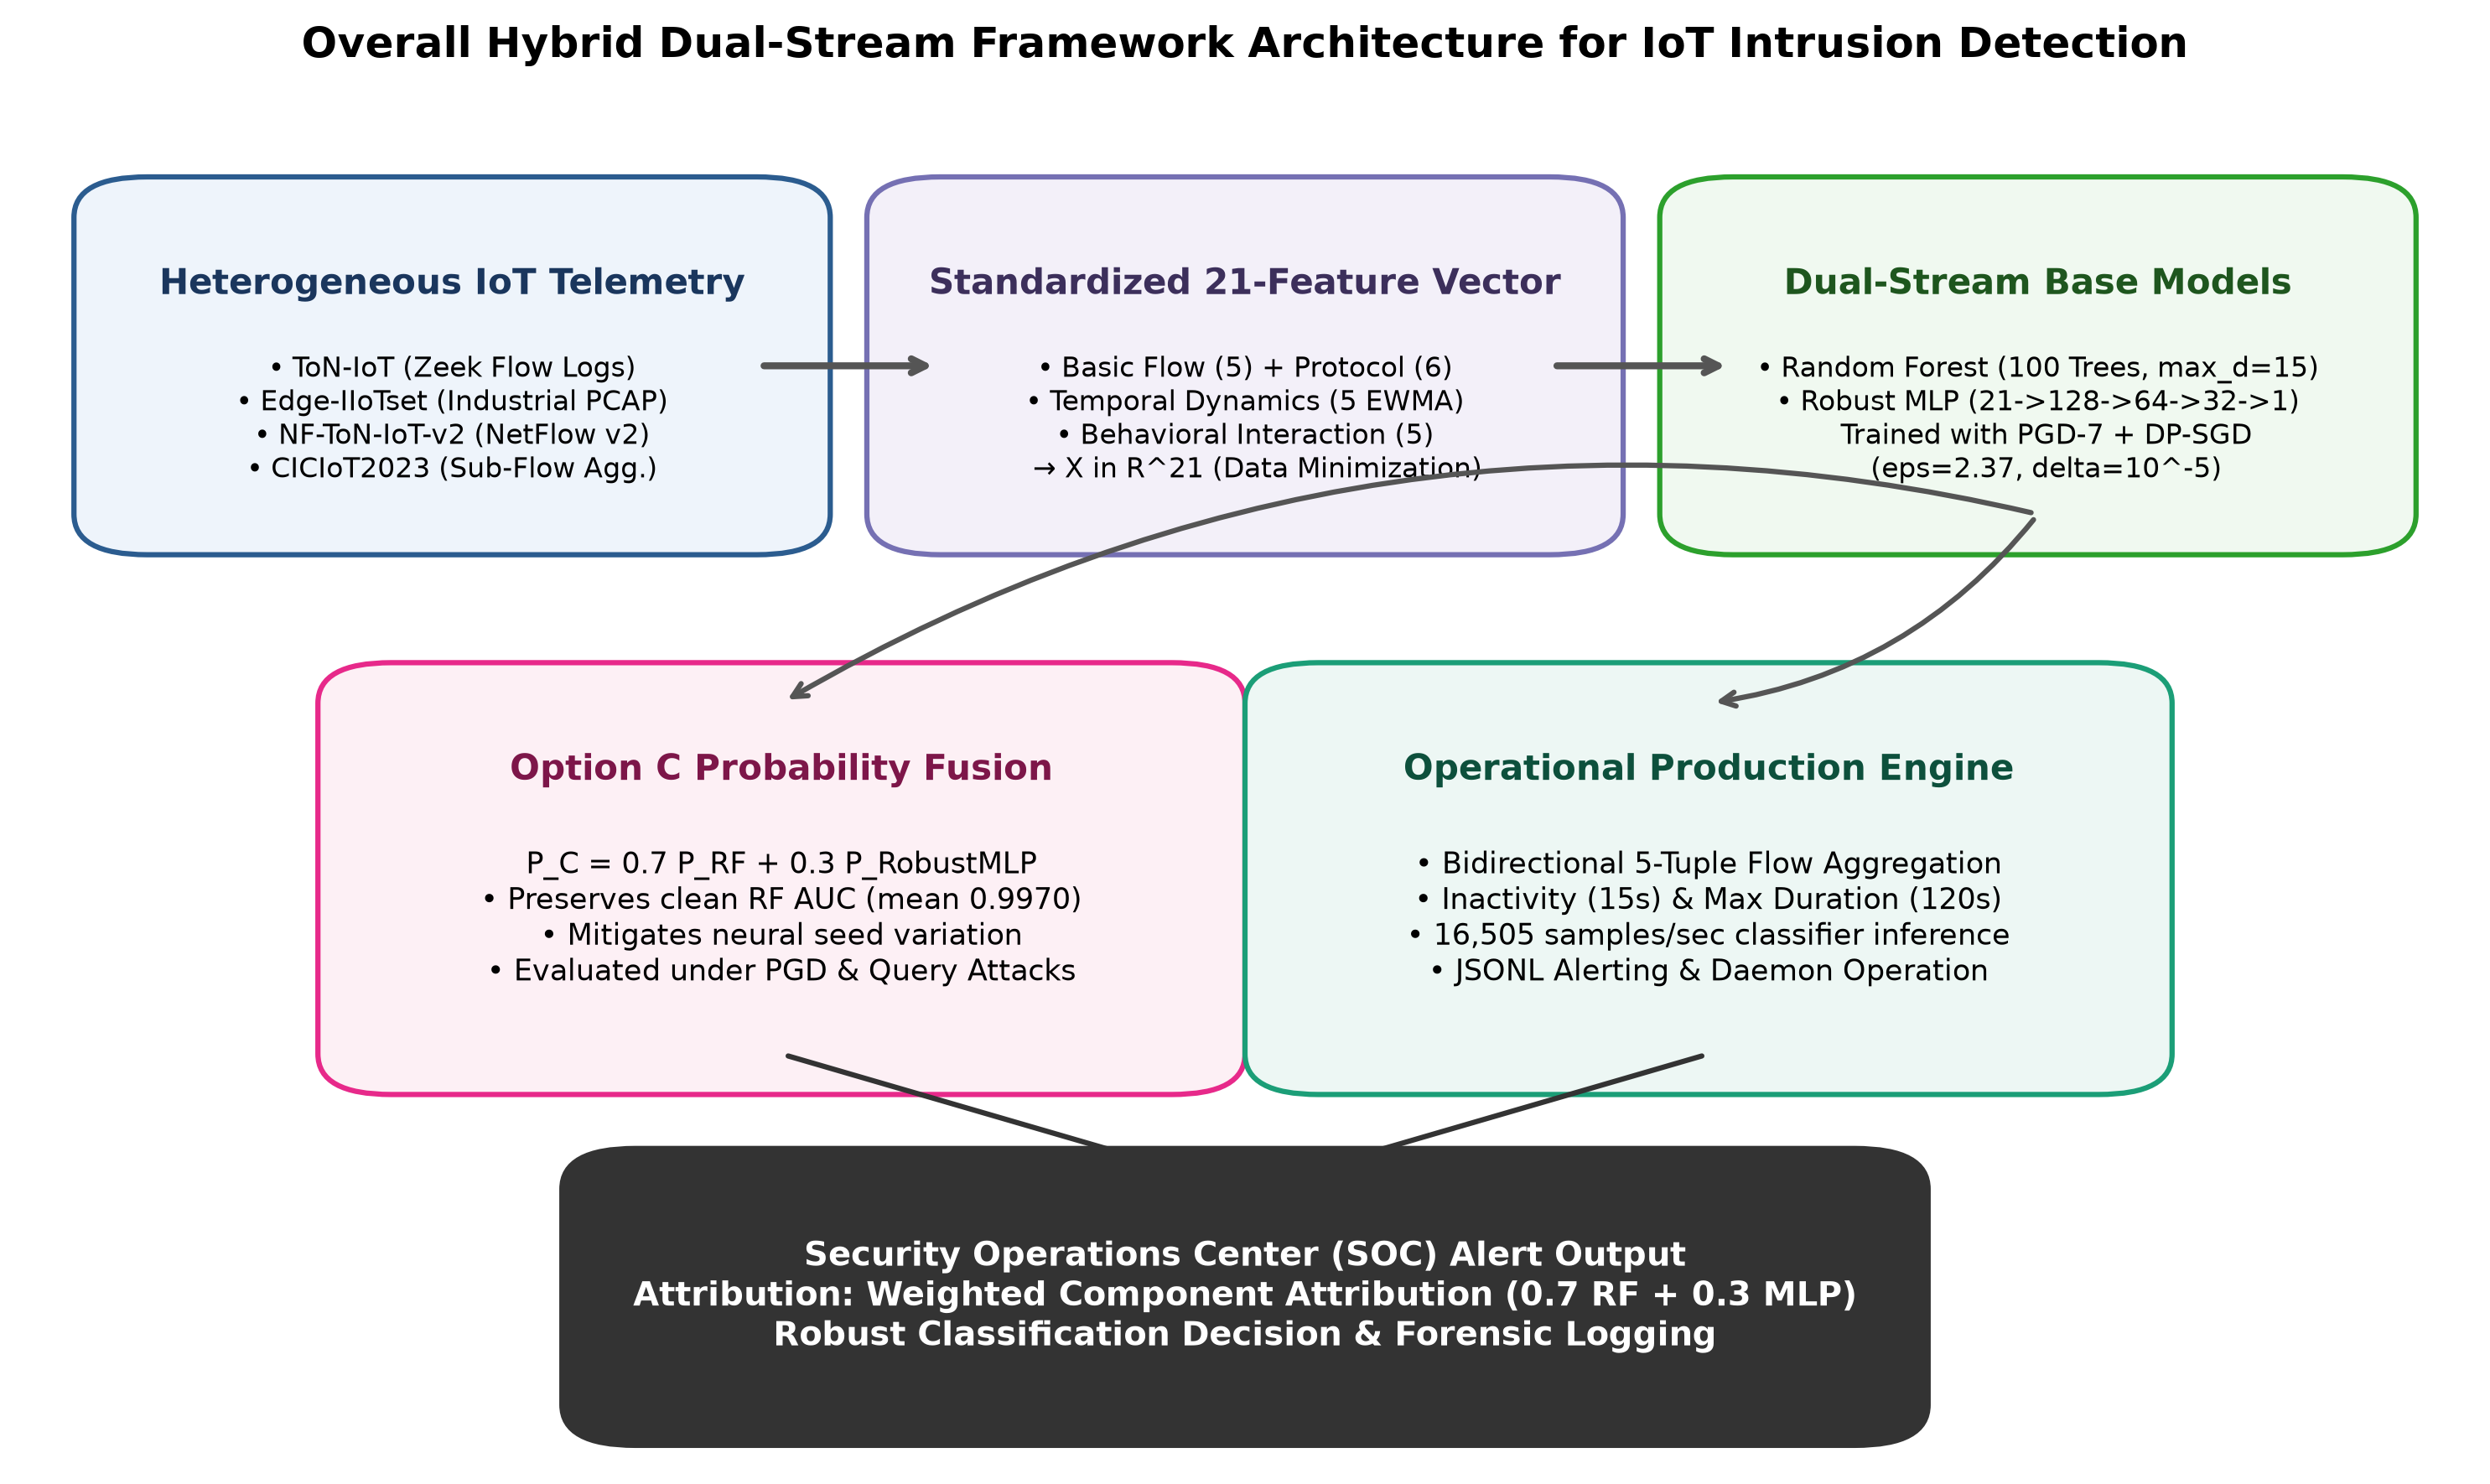
\includegraphics[width=0.92\textwidth]{figures/system_overview.png}
\caption{Overall hybrid dual-stream framework architecture for IoT intrusion detection, combining standardized 21-feature flow extraction, Random Forest classification, PGD+DP-SGD robust neural inference, Option~C probability fusion, and weighted attribution explainability.}
\label{fig:sys_overview}
\end{figure*}

\subsection{Standardized 21-Feature Flow Representation}
To satisfy privacy-preserving data minimization while ensuring cross-dataset compatibility, the framework rejects raw packet payload storage. Instead, incoming packets are aggregated into bidirectional network flows identified by the five-tuple:
\begin{equation}
\text{Flow ID} = (\text{IP}_{\text{src}}, \text{IP}_{\text{dst}}, \text{Port}_{\text{src}}, \text{Port}_{\text{dst}}, \text{Protocol})
\end{equation}
Flows are summarized into a uniform 21-dimensional continuous vector $\mathbf{x} \in \mathbb{R}^{21}$ categorized into four distinct functional tiers, as specified in Table~\ref{tab:feature_schema}.

\begin{table}[htbp]
\caption{Standardized 21-Feature Representation Schema}
\label{tab:feature_schema}
\centering
\begin{tabular}{llp{4.2cm}}
\toprule
\textbf{Feature Name} & \textbf{Category} & \textbf{Description \& Semantics} \\
\midrule
\texttt{flow\_duration} & Basic Flow & Total flow duration in seconds. \\
\texttt{flow\_bytes\_per\_sec} & Basic Flow & Total payload and header byte rate. \\
\texttt{flow\_pkts\_per\_sec} & Basic Flow & Packet transmission frequency. \\
\texttt{mean\_pkt\_size} & Basic Flow & Arithmetic mean of packet byte sizes. \\
\texttt{payload\_byte\_ratio} & Basic Flow & Ratio of forward to reverse byte volume. \\
\midrule
\texttt{pkt\_count\_ratio} & Protocol & Ratio of forward to reverse packet count. \\
\texttt{tcp\_syn\_ratio} & Protocol & Proportion of packets with TCP SYN flag set. \\
\texttt{proto\_tcp} & Protocol & One-hot indicator: TCP transport protocol. \\
\texttt{proto\_udp} & Protocol & One-hot indicator: UDP transport protocol. \\
\texttt{proto\_icmp} & Protocol & One-hot indicator: ICMP network protocol. \\
\texttt{proto\_other} & Protocol & One-hot indicator: Alternative protocol. \\
\midrule
\texttt{temporal\_iat\_mean} & Temporal & Mean packet inter-arrival time (s). \\
\texttt{temporal\_iat\_cv} & Temporal & Coefficient of variation of inter-arrival times. \\
\texttt{temporal\_flow\_rate\_ewma} & Temporal & EWMA of flow initiation rate ($\alpha=0.1$). \\
\texttt{temporal\_byte\_rate\_ewma} & Temporal & EWMA of host byte transmission rate. \\
\texttt{temporal\_syn\_rate\_ewma} & Temporal & EWMA of TCP SYN connection attempts. \\
\midrule
\texttt{behavioral\_dst\_diversity} & Behavioral & Unique destination IP count in active window. \\
\texttt{behavioral\_port\_entropy} & Behavioral & Shannon entropy of destination port usage. \\
\texttt{behavioral\_fanout\_ratio} & Behavioral & Ratio of outgoing to incoming flows. \\
\texttt{behavioral\_unanswered\_ratio} & Behavioral & Ratio of TCP connection requests without ACK. \\
\texttt{behavioral\_src\_activity\_ewma} & Behavioral & Cumulative EWMA of source host events. \\
\bottomrule
\end{tabular}
\end{table}

\subsection{Preprocessing Sensitivity and Locked Scaling}
During empirical auditing, we identified preprocessing as an acute source of model instability. Specifically, applying a logarithmic transform ($\log(1+x)$) prior to scaling dramatically alters baseline feature geometries compared to raw scaling. On Edge-IIoTset, standard MLP ROC-AUC shifted from $0.8443$ under raw features to $0.9820$ under $\log(1+x)$ preprocessing. Consequently, preprocessing cannot be treated as an arbitrary engineering choice; it constitutes an integral part of the model definition. To maintain strict experimental validity, all models in this study are locked to the canonical pipeline: raw features normalized via \texttt{RobustScaler} fitted exclusively on training flows, clamping outliers without logarithmic distortion.

\subsection{Dual-Stream Option C Ensemble Formulation}
The core detector combines two complementary learning paradigms:
\begin{enumerate}
    \item \textbf{Random Forest Stream}: An ensemble of 100 decorrelated decision trees~\cite{breiman2001random} with maximum depth constrained to 15. The Random Forest generates an attack probability:
    \begin{equation}
    P_{\text{RF}}(y=1 \mid \mathbf{x}) = \frac{1}{100} \sum_{t=1}^{100} P_t(y=1 \mid \mathbf{x})
    \end{equation}
    RF exhibits high stability, near-zero variance across initialization seeds, and near-perfect clean tabular classification.
    \item \textbf{Robust MLP Neural Stream}: A 4-layer fully connected architecture ($21 \to 128 \to 64 \to 32 \to 1$) with Batch Normalization, ReLU non-linearities, and Dropout ($p=0.2$). The neural network outputs an attack probability:
    \begin{equation}
    P_{\text{MLP}}(y=1 \mid \mathbf{x}) = \sigma(\mathbf{w}^T \mathbf{h}_3 + b)
    \end{equation}
    where $\sigma(z) = (1 + e^{-z})^{-1}$.
\end{enumerate}

Probability predictions from both streams are unified via Option~C weighted probability fusion:
\begin{equation}
P_{\text{Option C}}(y=1 \mid \mathbf{x}) = 0.7 \cdot P_{\text{RF}}(y=1 \mid \mathbf{x}) + 0.3 \cdot P_{\text{MLP}}(y=1 \mid \mathbf{x})
\label{eq:option_c_fusion}
\end{equation}
An alert is raised when $P_{\text{Option C}} \ge \tau$, where $\tau = 0.50$ serves as the default classification boundary and $\tau = 0.71$ serves as an operational high-confidence threshold.

\subsection{Joint Adversarial and Differentially Private Training}
The neural stream is trained under joint PGD adversarial regularization and Differential Privacy (DP-SGD). In each training mini-batch $B$, adversarial perturbations $\mathbf{\delta}$ are generated within an $L_\infty$ ball of radius $\epsilon = 0.10$ over 7 PGD iterations:
\begin{equation}
\mathbf{x}_{\text{adv}}^{k+1} = \Pi_{\mathbf{x} + S} \left( \mathbf{x}_{\text{adv}}^k + \alpha \cdot \text{sign}(\nabla_{\mathbf{x}} \mathcal{L}(\theta, \mathbf{x}_{\text{adv}}^k, y)) \right)
\end{equation}
where step size $\alpha = 0.025$, initial step $\mathbf{x}_{\text{adv}}^0 = \mathbf{x}$, and $S = \{ \mathbf{\delta} \in \mathbb{R}^{21} \mid \|\mathbf{\delta}\|_\infty \le 0.10, \mathbf{\delta}_{\text{protocol}} = 0 \}$. Crucially, one-hot protocol indicators are masked to zero perturbation ($\mathbf{\delta}_{\text{protocol}} = 0$), preserving legitimate network semantics.

To enforce Differential Privacy, per-sample gradients $\mathbf{g}_i = \nabla_\theta \mathcal{L}(\theta, \mathbf{x}_{i, \text{adv}}, y_i)$ are computed, clipped to maximum $L_2$ norm $C = 1.0$, and perturbed with calibrated Gaussian noise:
\begin{equation}
\tilde{\mathbf{g}} = \frac{1}{|B|} \left( \sum_{i \in B} \frac{\mathbf{g}_i}{\max\left(1, \frac{\|\mathbf{g}_i\|_2}{C}\right)} + \mathcal{N}(0, \sigma^2 C^2 \mathbf{I}) \right)
\end{equation}
with noise multiplier $\sigma = 1.0$ and clipping norm $C = 1.0$.

\textit{Privacy Accounting Scope}: Privacy consumption is tracked using the Opacus PRV accountant~\cite{mironov2017renyi}. Across $N_{\text{steps}} = 660$ training steps with Poisson subsampling probability $q = \frac{64}{4200} \approx 0.015238$, the neural stream achieves an audited privacy bound of $\varepsilon = 2.37$ at target $\delta = 10^{-5}$. We emphasize that this privacy guarantee applies \textbf{exclusively to the neural stream weights}. The Random Forest classifier and input feature scalers are constructed on training data without DP noise injection.

\subsection{Explainability via Attribution Aggregation}
Computing exact cooperative Shapley values for the fused predictor requires evaluating all $2^{21} = 2,097,152$ feature coalitions per flow. In empirical benchmarks, exact Shapley computation required $3.53$ seconds per single sample (roughly $1.37$ hours for 1,400 flows), rendering real-time operational XAI impossible. 

To overcome this, we implement \textbf{Weighted Component Attribution Aggregation} as a low-latency surrogate. Independent feature attributions $\mathbf{A}_{\text{RF}}$ (via TreeSHAP) and $\mathbf{A}_{\text{MLP}}$ (via expected gradients) are $L_1$-normalized and fused according to the Option~C weights:
\begin{equation}
\mathbf{A}_{\text{Option C}} = 0.7 \cdot \frac{\mathbf{A}_{\text{RF}}}{\|\mathbf{A}_{\text{RF}}\|_1} + 0.3 \cdot \frac{\mathbf{A}_{\text{MLP}}}{\|\mathbf{A}_{\text{MLP}}\|_1}
\label{eq:xai_surrogate}
\end{equation}
While this linear surrogate violates the strict game-theoretic Shapley additivity axiom (exhibiting a mean residual of $0.8348$ against exact fused KernelSHAP), it maintains high rank correlation ($\rho = 0.845$) and executes in sub-millisecond time.

\subsection{Operational Pipeline Implementation}
The operational pipeline is implemented in Python and packaged for Docker daemon execution. It incorporates:
\begin{itemize}
    \item \textbf{Packet Capture \& Parsing}: Scapy-based network sniffing supporting both live interface capture and offline PCAP replay.
    \item \textbf{Stateful Flow Aggregation}: Bidirectional 5-tuple table tracking packet sizes, TCP flags, and inter-arrival timestamps, with an active flow timeout of $15$ seconds and maximum flow duration of $120$ seconds.
    \item \textbf{Fault-Tolerant Alert Routing}: Prediction outcomes are streamed to structured JSONL logs and stdout, accompanied by Prometheus runtime telemetry.
\end{itemize}

\section{Experimental Setup}
\subsection{Benchmark Datasets}
The framework was evaluated across four established IIoT and IoT benchmark datasets:
\begin{enumerate}
    \item \textbf{Edge-IIoTset}~\cite{edge2024benchmarking}: Contemporary IIoT testbed telemetry containing real industrial automation protocols (Modbus, MQTT) and 14 attack classes.
    \item \textbf{NF-ToN-IoT-v2}~\cite{sarhan2021netflow}: Standardized NetFlow-v9 representation of the ToN-IoT telemetry.
    \item \textbf{ToN-IoT}~\cite{moustafa2020toniot}: Heterogeneous sensor data collected from IoT edge nodes and operating systems.
    \item \textbf{CICIoT2023}~\cite{ciciot2023dataset}: Large-scale IoT attack dataset encompassing 33 distinct attack profiles across 105 IoT devices.
\end{enumerate}
Each dataset was partitioned into chronological 60/20/20 train/validation/test splits (4,200 training, 1,400 validation, and 1,400 test flows; 7,000 flows total per dataset) to prevent temporal data leakage.

\subsection{Evaluated Threat Models}
We formalize three distinct attack configurations to evaluate evasion resilience:
\begin{enumerate}
    \item \textbf{Neural-Gradient Transfer PGD-10}: Perturbations are crafted using gradients of the robust neural stream:
    \begin{equation}
    \mathbf{x}_{\text{adv}} = \text{PGD}_{10}(\mathbf{x}; \nabla_{\mathbf{x}} \mathcal{L}_{\text{MLP}})
    \end{equation}
    and subsequently evaluated on the frozen Option~C ensemble. Perturbation budget is bounded by $\epsilon = 0.10$ ($L_\infty$).
    \item \textbf{Adaptive Surrogate Attack}: An attacker trains a differentiable multilayer neural surrogate $S_{\text{RF}}(\mathbf{x})$ to mimic the Random Forest probability surface ($R^2 = 0.948$ on validation). Gradients are backpropagated through the joint surrogate ensemble:
    \begin{equation}
    f_{\text{surr}}(\mathbf{x}) = 0.7 S_{\text{RF}}(\mathbf{x}) + 0.3 P_{\text{MLP}}(\mathbf{x})
    \end{equation}
    \item \textbf{Black-Box NES Query Attack}: A true black-box adversary with score-query access to the complete, deployed Option~C output probability $P_{\text{Option C}}(\mathbf{x})$, without access to model weights or gradients. The adversary employs Natural Evolution Strategies (NES) with antithetic Gaussian sampling ($\sigma=0.01$, 10 antithetic pairs = 20 directional queries per step) to estimate numerical score gradients and perform projected descent ($\alpha=0.025, \epsilon=0.10$) across query budgets of 100, 250, and 500 queries.
\end{enumerate}

\section{Empirical Results and In-Depth Analysis}

\subsection{Clean Detection Performance}
Table~\ref{tab:clean_detection} presents clean detection performance across all four datasets. Random Forest achieves exceptional standalone performance on tabular flow statistics (mean ROC-AUC $0.9976$). The DP-trained robust MLP exhibits lower standalone ROC-AUC (mean $0.8562$) due to gradient clipping and noise injection. However, the Option~C ensemble restores aggregate mean ROC-AUC to \textbf{0.9970} (Edge-IIoTset: 0.9988, NF-ToN-IoT-v2: 0.9927, ToN-IoT: 1.0000, CICIoT2023: 0.9965), matching or approaching pure RF accuracy while embedding neural defense.

\begin{table*}[tbp]
\caption{Clean Detection Performance Across Datasets (ROC-AUC and Macro F1 with 95\% Bootstrap Confidence Intervals)}
\label{tab:clean_detection}
\centering
\begin{tabular}{lcccccc}
\toprule
\textbf{Dataset} & \textbf{RF AUC [95\% CI]} & \textbf{Std MLP AUC} & \textbf{Rob MLP AUC} & \textbf{Option C AUC [95\% CI]} & \textbf{Option C Macro F1 [95\% CI]} \\
\midrule
Edge-IIoTset & 0.9995 [0.9988, 0.9999] & 0.8443 & 0.8002 & \textbf{0.9988} [0.9968, 0.9999] & 0.9751 [0.9657, 0.9836] \\
NF-ToN-IoT-v2 & 0.9940 [0.9896, 0.9978] & 0.8398 & 0.8299 & \textbf{0.9927} [0.9853, 0.9981] & 0.9285 [0.9134, 0.9427] \\
ToN-IoT & 1.0000 [1.0000, 1.0000] & 0.7745 & 0.8063 & \textbf{1.0000} [1.0000, 1.0000] & 1.0000 [1.0000, 1.0000] \\
CICIoT2023 & 0.9968 [0.9946, 0.9986] & 0.9776 & 0.9884 & \textbf{0.9965} [0.9943, 0.9983] & 0.9292 [0.9121, 0.9434] \\
\midrule
\textbf{Aggregate Mean} & \textbf{0.9976} & \textbf{0.8590} & \textbf{0.8562} & \textbf{0.9970} & \textbf{0.9582} \\
\bottomrule
\end{tabular}
\end{table*}

\subsection{Robust MLP Seed Sensitivity and Checkpoint Selection}
A central finding of this investigation is the severe seed sensitivity of PGD adversarial training on tabular data. While running an identical training configuration with a fixed seed produces 100\% bit-exact reproducible checkpoints, varying the initialization seed across 10 independent runs (seeds 42 through 51) yields drastically disparate adversarial robustness, as illustrated in Fig.~\ref{fig:multiseed_robustness} and Table~\ref{tab:multiseed}.

\begin{figure}[htbp]
\centering
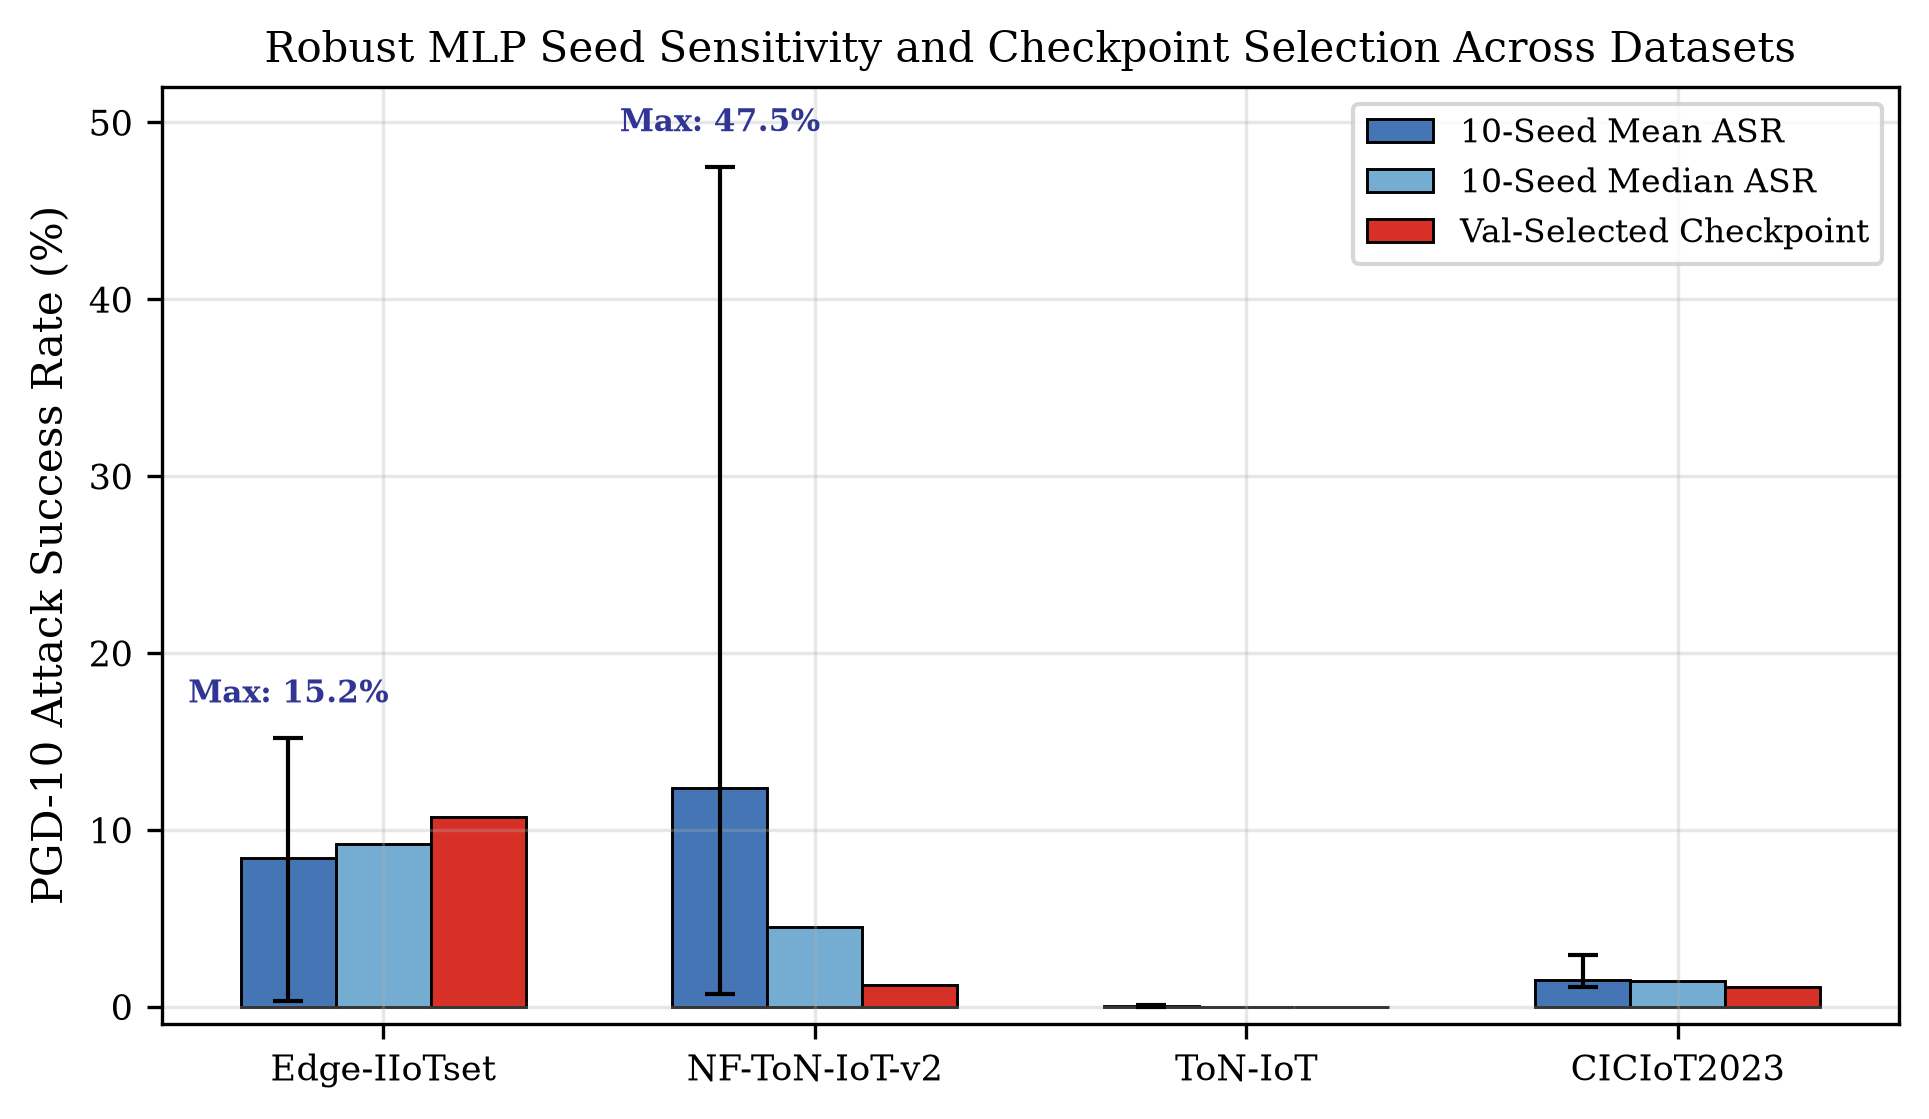
\includegraphics[width=\columnwidth]{figures/multiseed_robustness.png}
\caption{PGD-10 Attack Success Rate (ASR) distribution across 10 random initialization seeds compared against validation-selected checkpoints across benchmark datasets.}
\label{fig:multiseed_robustness}
\end{figure}

On NF-ToN-IoT-v2, the 10 seeds produced Option~C PGD-10 ASR values of: 44.8\% (seed 42), 1.2\% (seed 43), 4.5\% (seed 44), 4.1\% (seed 45), 47.5\% (seed 46), 0.7\% (seed 47), 5.0\% (seed 48), 6.9\% (seed 49), 4.5\% (seed 50), and 4.4\% (seed 51). The resulting distribution exhibits a mean of 12.36\%, a median of 4.50\%, and a massive standard deviation of 17.91\% (min 0.7\%, max 47.5\%). 

\begin{table}[htbp]
\caption{Multi-Seed Robustness Statistics and Validation Checkpoint Selection}
\label{tab:multiseed}
\centering
\begin{tabular}{lccccc}
\toprule
\textbf{Dataset} & \textbf{Mean ASR} & \textbf{Median} & \textbf{Std Dev} & \textbf{Min / Max} & \textbf{Val-Selected} \\
\midrule
Edge-IIoTset & 8.39\% & 9.20\% & 4.82\% & 0.30\% / 15.20\% & 10.70\% (Seed 44) \\
NF-ToN-IoT-v2 & 12.36\% & 4.50\% & 17.91\% & 0.70\% / 47.50\% & \textbf{1.20\%} (Seed 43) \\
ToN-IoT & 0.01\% & 0.00\% & 0.03\% & 0.00\% / 0.10\% & 0.00\% (Seed 42) \\
CICIoT2023 & 1.51\% & 1.45\% & 0.52\% & 1.10\% / 2.90\% & 1.10\% (Seed 42) \\
\bottomrule
\end{tabular}
\end{table}

\textit{Evaluation of Checkpoint Selection}: To mitigate this instability, we implemented validation-based checkpoint selection:
\begin{equation}
\text{Score}_{\text{val}} = \text{AUC}_{\text{val}} - 1.0 \cdot \text{ASR}_{\text{val}}
\end{equation}
without exposing test set labels. For NF-ToN-IoT-v2, validation selection successfully isolated seed 43, achieving a test ASR of \textbf{1.20\%}. However, on Edge-IIoTset, the same selection heuristic chose seed 44 with a test ASR of $10.70\%$, underperforming the 10-seed baseline mean of $8.39\%$. This proves that checkpoint selection is a domain-dependent mitigation rather than a universal guarantee.

\subsection{Threat Model Realities: Transfer vs. Direct Query Optimization}
Table~\ref{tab:adversarial_threat_models} and Fig.~\ref{fig:blackbox_attack} contrast evasion rates across the three evaluated threat models. Under neural-gradient transfer (PGD-10), Option~C reports an apparent ASR of only 6.51\% on NF-ToN-IoT-v2 and 5.35\% on Edge-IIoTset (excluding clean misclassifications). However, this apparent robustness is an artifact of gradient transfer: the Random Forest is non-differentiable, so its true decision boundaries are never directly targeted.

\begin{figure}[htbp]
\centering
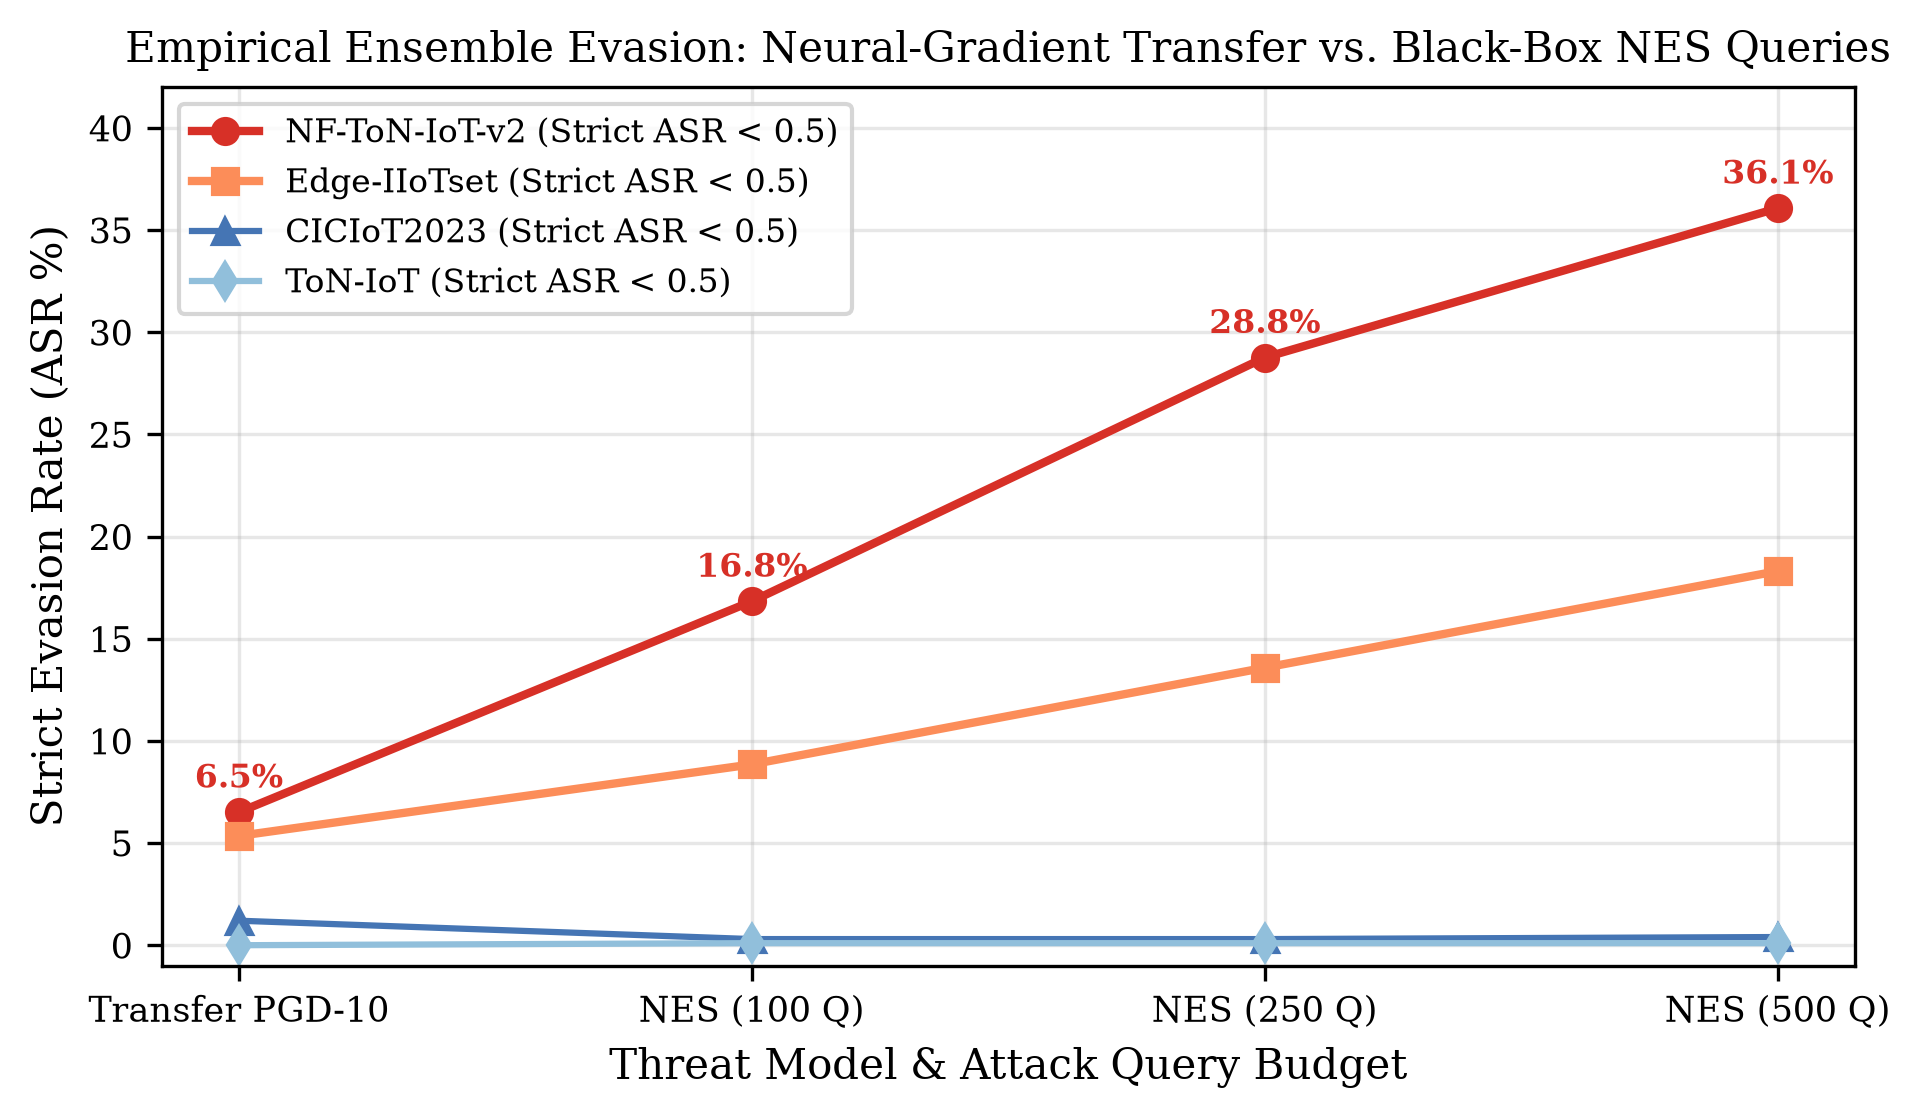
\includegraphics[width=\columnwidth]{figures/blackbox_query_attack.png}
\caption{Empirical ensemble evasion rate (ASR \%) under neural-gradient transfer versus black-box Natural Evolution Strategies (NES) query attacks across query budgets.}
\label{fig:blackbox_attack}
\end{figure}

When subjected to the black-box Natural Evolution Strategies (NES) attack optimizing directly against the fused Option~C score, evasion rates escalate monotonically with query budget. On NF-ToN-IoT-v2, strict ASR ($P_C < 0.50$) increases from 16.83\% (100 queries) to 28.76\% (250 queries) and reaches \textbf{36.07\%} at 500 queries. Under the operational detection threshold ($\tau = 0.71$), evasion reaches \textbf{83.90\%}. Similarly, on Edge-IIoTset, strict evasion climbs from 5.35\% (transfer) to \textbf{18.31\%} (500 queries). These empirical findings demonstrate that neural-gradient transfer substantially understates the empirical evasion risk of hybrid ensembles.

\begin{table*}[tbp]
\caption{Ensemble Adversarial Evasion Across Evaluated Threat Models ($\epsilon=0.10$)}
\label{tab:adversarial_threat_models}
\centering
\begin{tabular}{lcccccc}
\toprule
\textbf{Dataset} & \textbf{Transfer PGD-10} & \textbf{Adaptive Surrogate} & \textbf{NES (100 Queries)} & \textbf{NES (250 Queries)} & \textbf{NES (500 Queries)} & \textbf{NES Oper. ($\tau=0.71$)} \\
\midrule
Edge-IIoTset & 5.35\% & 11.80\% & 8.85\% & 13.58\% & \textbf{18.31\%} & 100.0\% ($N=5$) \\
NF-ToN-IoT-v2 & 6.51\% & 5.90\% & 16.83\% & 28.76\% & \textbf{36.07\%} & \textbf{83.90\%} \\
ToN-IoT & 0.00\% & 0.00\% & 0.10\% & 0.10\% & 0.10\% & 1.20\% \\
CICIoT2023 & 1.20\% & 1.10\% & 0.30\% & 0.30\% & 0.40\% & 33.06\% \\
\bottomrule
\end{tabular}
\end{table*}

\subsection{Fusion-Weight Analysis and Pareto Qualification}
We conducted an exhaustive ablation sweep of the Random Forest fusion weight $w_{\text{RF}} \in [0.0, 1.0]$ in increments of $0.10$, as detailed in Table~\ref{tab:fusion_sweep} and Fig.~\ref{fig:fusion_tradeoff}. 

\begin{figure}[htbp]
\centering
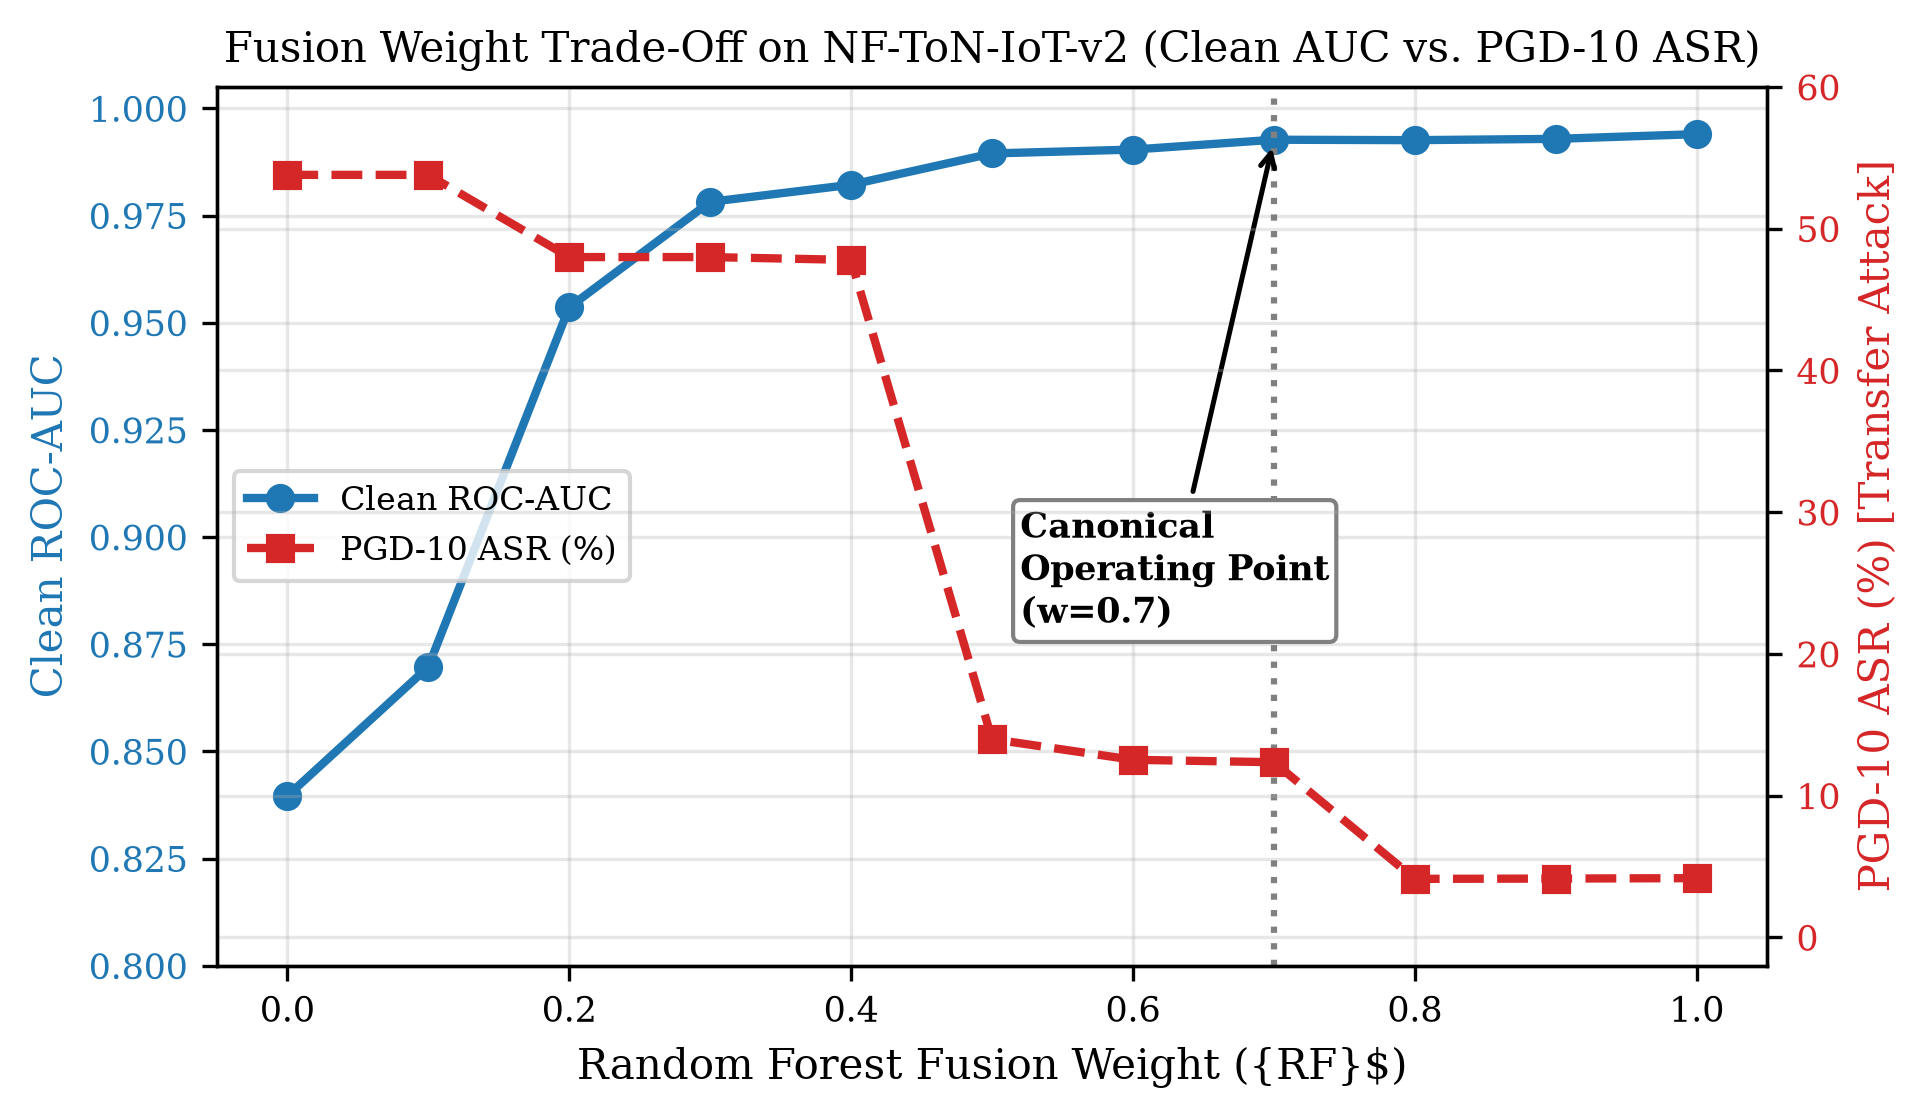
\includegraphics[width=\columnwidth]{figures/fusion_weight_tradeoff.png}
\caption{Fusion weight ablation sweep on NF-ToN-IoT-v2, illustrating the trade-off between clean detection ROC-AUC and transfer PGD-10 ASR as $w_{\text{RF}}$ varies from 0.0 to 1.0.}
\label{fig:fusion_tradeoff}
\end{figure}

The empirical results refute claims that $0.7/0.3$ is a globally optimal Pareto point. On NF-ToN-IoT-v2 across 10 seeds, mean ASR at $w_{\text{RF}}=0.7$ is $12.36\%$, whereas $w_{\text{RF}}=0.8$ achieves a substantially lower ASR of $4.13\%$ while maintaining clean ROC-AUC at $0.9926$. On CICIoT2023, clean ROC-AUC and ASR remain nearly identical across $w_{\text{RF}} \in [0.7, 1.0]$ ($0.9964$ vs. $0.9968$). Furthermore, because the evaluation attack utilized neural gradients, the sweep represents an empirical accuracy-robustness trade-off under a fixed neural-gradient protocol rather than a true security Pareto frontier. The $0.7/0.3$ configuration is therefore correctly framed as an \textbf{empirically evaluated operating point} providing high clean accuracy and balanced robustness.

\begin{table}[htbp]
\caption{Fusion Weight ($w_{\text{RF}}$) Ablation Sweep on NF-ToN-IoT-v2 (10-Seed Means)}
\label{tab:fusion_sweep}
\centering
\begin{tabular}{ccccc}
\toprule
$w_{\text{RF}}$ & $w_{\text{MLP}}$ & \textbf{Clean ROC-AUC} & \textbf{Transfer PGD ASR} & \textbf{Macro F1} \\
\midrule
0.0 & 1.0 & 0.8396 & 53.80\% & 0.5784 \\
0.2 & 0.8 & 0.9536 & 48.00\% & 0.8718 \\
0.4 & 0.6 & 0.9822 & 47.80\% & 0.9156 \\
0.5 & 0.5 & 0.9895 & 13.99\% & 0.9265 \\
0.6 & 0.4 & 0.9904 & 12.53\% & 0.9841 \\
\textbf{0.7} & \textbf{0.3} & \textbf{0.9927} & \textbf{12.36\%} & \textbf{0.9859} \\
0.8 & 0.2 & 0.9926 & 4.13\% & 0.9877 \\
0.9 & 0.1 & 0.9929 & 4.15\% & 0.9885 \\
1.0 & 0.0 & 0.9940 & 4.18\% & 0.9903 \\
\bottomrule
\end{tabular}
\end{table}

\subsection{Differential Privacy Analysis}
Table~\ref{tab:dp_analysis} details the privacy-utility-robustness trade-off for the neural stream across noise multipliers $\sigma \in \{0.0, 0.5, 1.0, 2.0\}$ at target $\delta = 10^{-5}$. At $\sigma=1.0$, the Opacus PRV accountant confirms an audited privacy budget of $\varepsilon = 2.37$, sustaining clean neural ROC-AUC at $0.8541$. Increasing noise to $\sigma=2.0$ tightens privacy to $\varepsilon = 0.80$ at the cost of nominal utility ($0.8284$).

\begin{table}[htbp]
\caption{DP-SGD Privacy Loss and Robustness on NF-ToN-IoT-v2 ($\delta=10^{-5}$)}
\label{tab:dp_analysis}
\centering
\begin{tabular}{cccc}
\toprule
\textbf{Noise Multiplier ($\sigma$)} & \textbf{Audited $\varepsilon$} & \textbf{Neural Clean AUC} & \textbf{PGD-10 ASR} \\
\midrule
0.0 (Non-private) & $\infty$ & 0.9763 & 1.5\% \\
0.5 & 15.85 & 0.8865 & 2.5\% \\
\textbf{1.0 (Canonical)} & \textbf{2.37} & \textbf{0.8541} & \textbf{47.7\%} \\
2.0 & 0.80 & 0.8284 & 47.8\% \\
\bottomrule
\end{tabular}
\end{table}

\subsection{Explainability and Feature Attribution}
Table~\ref{tab:xai_attribution} records the top three contributing features identified by Weighted Component Attribution Aggregation across attack families. Temporal and behavioral dynamics dominate threat attribution: on Edge-IIoTset injection attacks, \texttt{behavioral\_unanswered\_ratio} ($0.219$) and \texttt{behavioral\_port\_entropy} ($0.189$) contribute over 40\% of attribution weight, confirming that the multi-level representation captures distinctive topological signatures.

\begin{table}[htbp]
\caption{Top Attributed Features per Attack Family (Option C Surrogate XAI)}
\label{tab:xai_attribution}
\centering
\begin{tabular}{llp{4.8cm}}
\toprule
\textbf{Dataset} & \textbf{Attack Family} & \textbf{Top-3 Attributed Features (Weight)} \\
\midrule
Edge-IIoTset & Injection & \texttt{unanswered\_ratio} (0.219), \texttt{port\_entropy} (0.189), \texttt{dst\_diversity} (0.137) \\
NF-ToN-IoT-v2 & Scanning & \texttt{mean\_pkt\_size} (0.138), \texttt{flow\_rate\_ewma} (0.119), \texttt{flow\_bytes/s} (0.114) \\
ToN-IoT & Backdoor & \texttt{src\_activity\_ewma} (0.303), \texttt{syn\_rate\_ewma} (0.153), \texttt{flow\_duration} (0.111) \\
CICIoT2023 & DDoS & \texttt{src\_activity\_ewma} (0.241), \texttt{mean\_pkt\_size} (0.137), \texttt{iat\_mean} (0.124) \\
\bottomrule
\end{tabular}
\end{table}

\subsection{Host Runtime Latency and Pipeline Benchmark}
Offline classifier inference throughput was benchmarked on a single Intel Core CPU host across batch sizes $N \in \{1, \dots, 1024\}$, as reported in Table~\ref{tab:runtime_benchmarks}. At batch size $N=1024$, the classification engine achieves \textbf{16,504.7 samples/sec} with a per-sample latency of $0.0606$\,ms. 

\textit{Operational Throughput Distinction}: We explicitly distinguish this offline classifier benchmark from end-to-end network packet throughput. In live operation, packet sniffing (via Scapy), IP/TCP decoding, stateful 5-tuple flow aggregation, and feature derivation introduce processing overhead that bounds live pipeline throughput below the offline classifier ceiling. Functional end-to-end integrity was confirmed via an integration smoke test (4 packets $\to$ 2 flows $\to$ 1 anomaly alert, 0 errors) and validated by 174 passing regression tests.

\begin{table}[htbp]
\caption{Single-CPU Classifier Inference Latency and Throughput}
\label{tab:runtime_benchmarks}
\centering
\begin{tabular}{rccc}
\toprule
\textbf{Batch ($N$)} & \textbf{Batch Latency (ms)} & \textbf{Per-Sample (ms)} & \textbf{Throughput (samples/s)} \\
\midrule
1 & 69.40 & 69.4000 & 14.4 \\
32 & 54.86 & 1.7143 & 583.3 \\
64 & 46.51 & 0.7267 & 1,376.1 \\
128 & 46.68 & 0.3647 & 2,742.3 \\
256 & 61.11 & 0.2387 & 4,189.0 \\
512 & 60.88 & 0.1189 & 8,409.5 \\
\textbf{1024} & \textbf{62.04} & \textbf{0.0606} & \textbf{16,504.7} \\
\bottomrule
\end{tabular}
\end{table}

\section{Research Scope, Limitations, and Threats to Validity}
To uphold rigorous scientific integrity, Table~\ref{tab:limitations_matrix} delineates the validated scope, explicit boundaries, and remaining limitations of our study.

\begin{table*}[tbp]
\caption{Systematic Scope Matrix: Validated Contributions, Evidence Boundaries, and Limitations}
\label{tab:limitations_matrix}
\centering
\begin{tabular}{p{3.2cm}p{6.8cm}p{6.5cm}}
\toprule
\textbf{Dimension} & \textbf{Validated Empirical Finding} & \textbf{Threats to Validity \& Candid Scope Limitations} \\
\midrule
Adversarial Robustness Guarantee & PGD adversarial training improves neural robustness on select seeds; Option~C reduces transfer PGD ASR to 1.20\% on NF-ToN-IoT-v2. & Not an architectural guarantee; acute seed sensitivity (ASR up to 47.5\%); direct black-box query attacks achieve 36.07\% evasion. \\
\midrule
Ensemble Optimality & $w_{\text{RF}}=0.7$ provides high clean AUC (0.9970) and balanced defense on evaluated checkpoints. & Not globally optimal; $w_{\text{RF}}=0.8$ yields lower ASR on NF-ToN-IoT-v2; P4 represents an empirical trade-off under a fixed attack protocol. \\
\midrule
Differential Privacy & Opacus PRV accountant proves $(\varepsilon=2.37, \delta=10^{-5})$ DP-SGD bound for neural branch ($N_{\text{steps}}=660, q=0.0152$). & DP applies strictly to neural branch weights; Random Forest, scalers, and live packet capture do not satisfy $(\varepsilon, \delta)$-DP. \\
\midrule
Explainability (XAI) & Weighted Component Attribution Aggregation ($0.7\,\text{RF} + 0.3\,\text{MLP}$) provides real-time ranking ($\rho = 0.845$). & Violates Shapley additivity axiom; not exact SHAP for the fused model; exact $2^{21}$ coalition calculation is computationally intractable. \\
\midrule
Runtime Throughput & Single-CPU host classifier inference achieves 16,505 samples/sec (0.0606\,ms/sample) at batch $N=1024$. & Benchmark measures offline classifier inference only; excludes Scapy capture, flow aggregation, and network I/O latency. \\
\midrule
Domain Generalization & Evaluated on chronological 60/20/20 splits across 4 diverse benchmark datasets. & Evaluation does not prove zero-shot transfer to completely unseen physical IoT testbed topologies or unobserved protocols. \\
\bottomrule
\end{tabular}
\end{table*}

\section{Conclusion}
This paper presented an integrated dual-stream ensemble framework for IoT and IIoT intrusion detection, uniting high clean classification accuracy, adversarial robustness, differential privacy, and explainability over a standardized 21-feature representation. By combining a Random Forest with an adversarially trained, differentially private MLP via Option~C fusion, the system achieves a mean clean ROC-AUC of 0.9970 across four benchmark datasets.

Rather than asserting unverified robustness guarantees, our study systematically exposes the critical limitations of standard adversarial training in tabular network domains. We demonstrate that robust MLP training is highly seed-sensitive (ASR fluctuating from 0.7\% to 47.5\% across identical runs), that validation checkpoint selection is a conditional heuristic, and that gradient transfer attacks substantially understate ensemble vulnerability compared to direct black-box query optimization (36.07\% evasion under 500 NES queries). By transparently bounding differential privacy to the neural stream ($\varepsilon=2.37$), defining XAI as a low-latency surrogate, and decoupling classifier inference (16,505 samples/sec) from live network ingestion, this work establishes a rigorous, reproducible, and defensible foundation for secure machine learning in IoT environments.

\bibliographystyle{IEEEtran}
\bibliography{references}

\end{document}
